\chapter{検証実験}\label{chap:experiment}

\section{概要}
本論文で提案する個人認証システムについて,3つの評価実験を行った.
それぞれの実験は,時間的な制約から予備実験,本実験などの形式で行うことをせず,一度に行った.

\subsection{実験手順}
以降の節のそれぞれの実験は第\ref{subsec:selectSecret}節にて挙げた3つの実装(以降,「パターン」と記載する)に対応しており,それぞれのパターンは多要素化手法として評価するために認証操作の後に4桁のPINによる認証操作を追加した.
そこに「PINの桁数を一桁増やし,5桁にしたものを秘密情報とする」パターンを追加し,計4パターンで相互に比較を行った.
各パターンの実験は一つにつき8日間にわたって実施,その間に設定した日から数えて,0日目(設定直後),1日目,3日目,8日目の4回の認証試行を行った.
それぞれのパターンで実験中の期間は重複せず,順番は偏りのないように設定し,そのスケジュールにそって全実験を実施した.
スケジュールは4つのパターンの組み合わせであり,その総数は$ {}_4 P _4 $の式で表される.
本実験ではこれら全てに固有の番号(以降,「スケジュール番号」と記載する)を付録\ref{apdx:schedule}の通り割り振って管理する.

\subsubsection{初回実験説明・導入}
\begin{enumerate}
  \item 実験担当者が実験の目的・注意事項・免責事項を説明する.この手順は付録\ref{apdx:experiment}の実験説明資料と操作説明資料を用いて行う.
  \item 不明な点があれば質問してもらう.
  \item 被験者のスケジュールを決定し,それに合わせて提案システムを実装したアプリケーションソフトウェア(以降「Notifauth」と記載する)のソースコードにスケジュール番号を登録する.
  \item 実験担当者の開発用端末と被験者の携帯端末を接続し,Notifauthをインストールする\footnote{ここでAppleの開発者用アカウントと被験者の端末の紐付けを行う}.
  \item 実際にNotifauthを操作し,全てのパターンでひと通りの秘密情報設定と認証操作を行ってもらう.
  \item その後,Notifauth内の全ての保存されたデータを初期化し,スケジュールに沿ったパターンのみ設定を行ってもらうことで実験開始とする.
  \item 上記手順で設定したパターンについて認証操作を行ってもらう.
  \item この段階で実験データを送信してもらい,該当データの受信を実験担当者が確認ののち,初回実験説明・導入の終了とする.
\end{enumerate}

\subsubsection{試行手順}
\begin{enumerate}
  \item トップ画面で,試行したいパターンをセレクタで選択し,「Test」をタップする.
  \item ``PIN Mode''以外の場合,ロック画面を模した画面が表示され,秘密情報に当てはまると思われるツイートを見つけ,そのセルをスライドする.
  \item PINの入力画面が表示され,``PIN Mode''であれば5桁,それ以外のパターンであれば4桁のPINを入力する.
  \item 結果画面が表示されるので,「Home」をタップする.
\end{enumerate}

\subsubsection{結果送信手順}
\begin{enumerate}
  \item トップ画面で「Send」をタップすると,iOS標準のメール送信画面が開くので,何も編集を行わずに送信する.
  \item ここで仮にiOSへ自分のメール情報(送信サーバ,アカウントなど)が登録されていない場合以下の手順を行う
  \begin{enumerate}
    \item 「Send」をタップせず,トップ画面下部の「copy experiment data on clipboard」をタップする.
    \item クリップボードにデータがコピーされているので,メールアプリに貼り付けて実験担当者のメールアドレスへ送信する.
  \end{enumerate}
\end{enumerate}

\subsection{被験者}
男性12名,女性3名の計15名が実験を行った.
うち本学の学生は5名であった.
性別や年齢は表\ref{tab:participants}の通りである.
全ての検証実験を終了したのは12人で,そのうち最終アンケートに答えたのは○人である.
中間アンケートには○人が回答した.

\begin{table}[ht]
  \begin{minipage}{0.3\hsize}
    \begin{center}
      \small
      \begin{tabular}{|l|r|} \hline
        \multicolumn{2}{|l|}{性別} \\ \hline
        男性 & 15 \\
        女性 & 3 \\ \hline
      \end{tabular}
    \end{center}
  \end{minipage}
  \begin{minipage}{0.3\hsize}
    \begin{center}
      \small
      \begin{tabular}{|l|r|} \hline
        \multicolumn{2}{|l|}{年齢} \\ \hline
        10代 & 0 \\
        20代 & 12 \\
        30代 & 2 \\
        40代 & 1 \\
        50代以上 & 0 \\ \hline
      \end{tabular}
    \end{center}
  \end{minipage}
  \begin{minipage}{0.3\hsize}
    \begin{center}
      \small
      \begin{tabular}{|l|r|} \hline
        \multicolumn{2}{|l|}{1日の平均ツイート数} \\ \hline
        0〜1 & 0 \\
        2〜10 & 0 \\
        11〜50 & 0 \\
        50〜100 & 0 \\
        100〜 & 0 \\ \hline
      \end{tabular}
    \end{center}
  \end{minipage}
  \caption{被験者の特性}
  \label{tab:participants}
\end{table}

\section{SNSの情報を利用することに関する評価実験}\label{sec:vsTweet}
\subsection{目的}
本実験では,SNSの情報を利用することで,従来のPINを一桁増やした認証と比較し,どれだけ利便性と安全性を向上させることができるかの評価を行う.
本実験で評価対象とするパターンとして,``Manual Mode''を採用する.
アプリケーションを用いた実験では以下の3指標を測定する.

\begin{itemize}
  \item 短期の記憶保持
    \begin{description}
      \item[測定方法] 0日目,1日目,3日目の認証成功率を比較し,相関をみる.
      \item[意義] 短期に記憶が保持できなければ,使用の継続が難しくなってしまうため.
      \item[目標] 5桁のPIN認証よりも平均での認証率が高く,日数によって認証成功率が落ちにくいことを目指す.
    \end{description}
  \item 長期の記憶保持
    \begin{description}
      \item[測定方法] 3日目と8日目の認証成功率を比較し,相関をみる.
      \item[意義] 長期に記憶が保持できなければ,該当の認証を使わない期間が存在した際に認証できず,ユーザに秘密情報の再設定などの負担を与えてしまうため.
      \item[目標] 5桁のPIN認証よりも平均での認証率が高く,日数によって認証成功率が落ちにくいことを目指す.
    \end{description}
  \item 認証時間
    \begin{description}
      \item[測定方法] 認証操作の画面が表示されてから,認証を終えるまでの時間を計測する.認証の成否は問わないものとする.
      \item[意義] 認証操作に時間がかかりすぎてしまっては,携帯端末は一日に何度も認証を行うという仮定のもとでは,ユーザをいらいらさせてしまったりして,利便性を損ねてしまうため.
      \item[目標] 5桁のPIN認証よりも認証時間が短いことを目指す.
    \end{description}
\end{itemize}

また,有意差はWhelchのt検定を用いる(この場合標本が正規分布であることは自明とした[FIX: 自明じゃないのでマン・ホイットニーのU検定にするかも])

\subsection{方法}
被験者実験により各試行の成功と失敗,認証にかかった時間を収集する.
また,付録の\ref{apdx:interimEnquete}や\ref{apdx:finalEnquete}にある通り,被験者には使用パターンについて5段階のリッカート尺度を使った質問に答えてもらい,さらに既に8日間の試行が終了している他パターンとの比較もしてもらう.

\subsection{結果}
本実験の結果を述べる.
試行のタイミングが1日程度前後した被験者が存在したため,1〜2日目を1日目,3〜6日目におこなったものを3日目,7〜8日目に行ったものを8日目の試行とした.
\begin{table}[ht]
  \begin{center}
    \small
    \begin{tabular}{|r|r|r|} \hline
      経過日数 & 認証成功率(\%) & 認証時間(秒)\\ \hline
      0 & 90.0 & 17.05 \\
      1〜2 & 88.9 & 11.86 \\
      3〜6 & 88.9 & 9.82 \\
      7〜8 & 100.0 & 10.11 \\ \hline \hline
      平均 & 91.89 & 12.34 \\
      標準偏差 & 4.67 & 9.56 \\ \hline
    \end{tabular}
  \end{center}
  \caption{Manual Modeにおける各経過日数ごとの認証成功率と認証時間の変化}
  \label{tab:manual.data}
\end{table}

\begin{figure}[ht]
  \begin{center}
    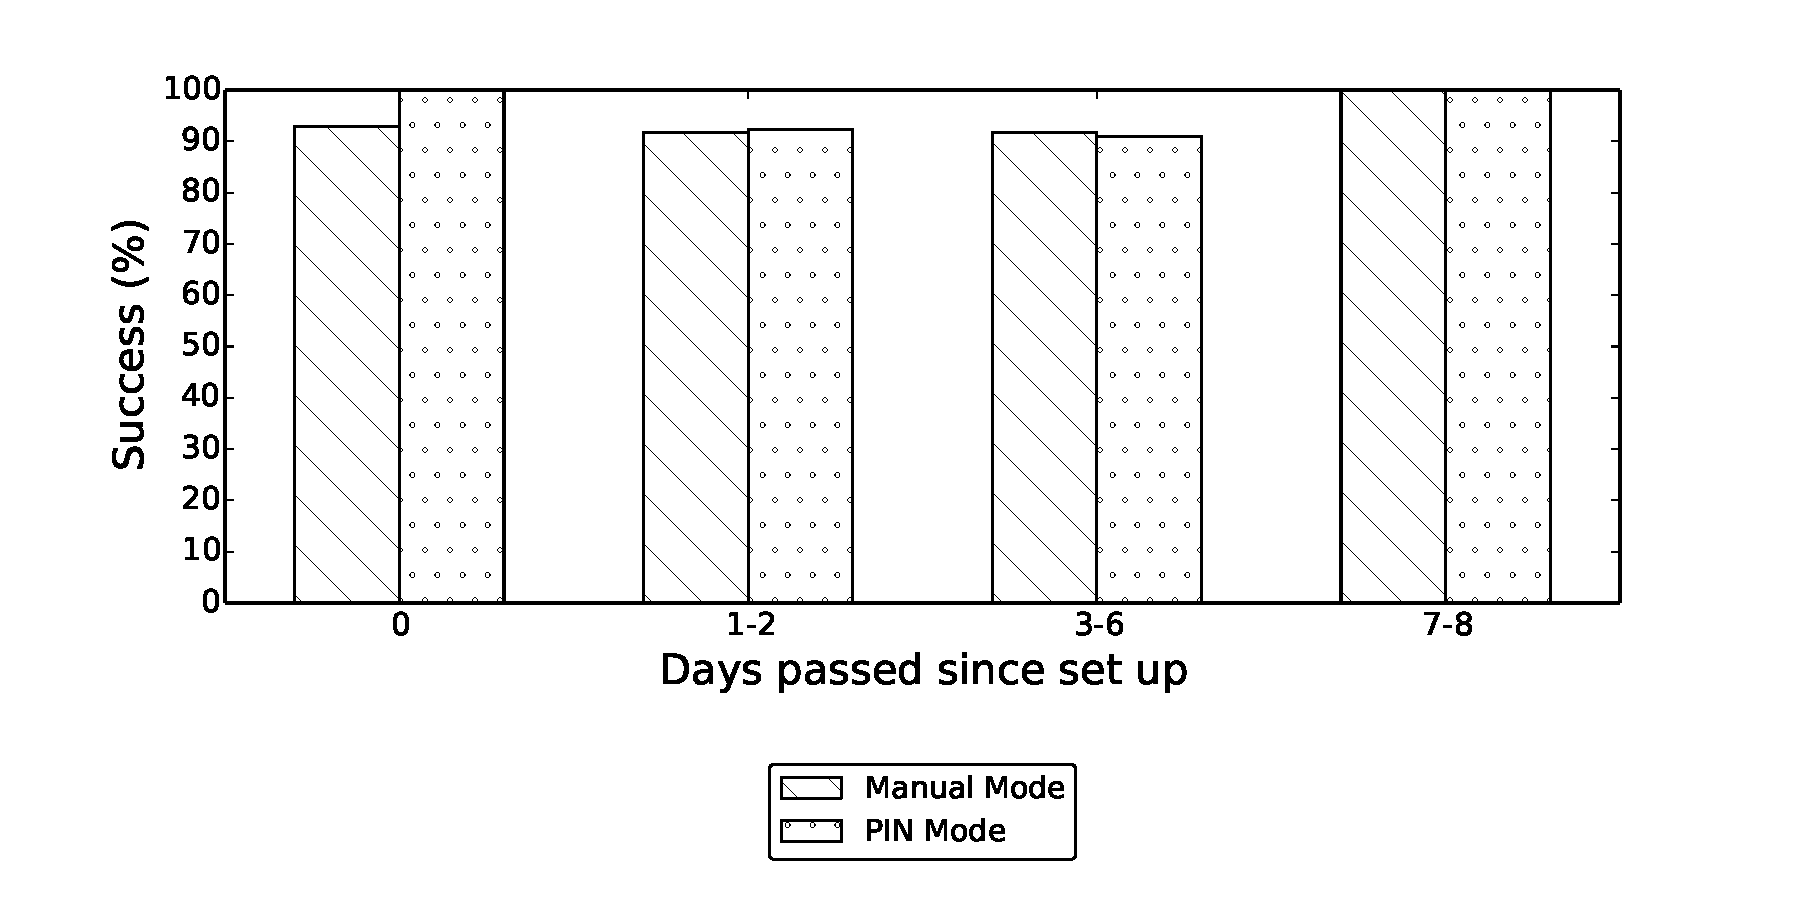
\epsfig{file=resource/ex_manual_vs_pin_rate.pdf,scale=0.5}
  \end{center}
  \caption{Manual ModeとPIN Modeにおける設定時からの経過日数ごとの認証成功率}
  \label{fig:ex_manual_vs_pin_rate}
\end{figure}

\begin{figure}[ht]
  \begin{center}
    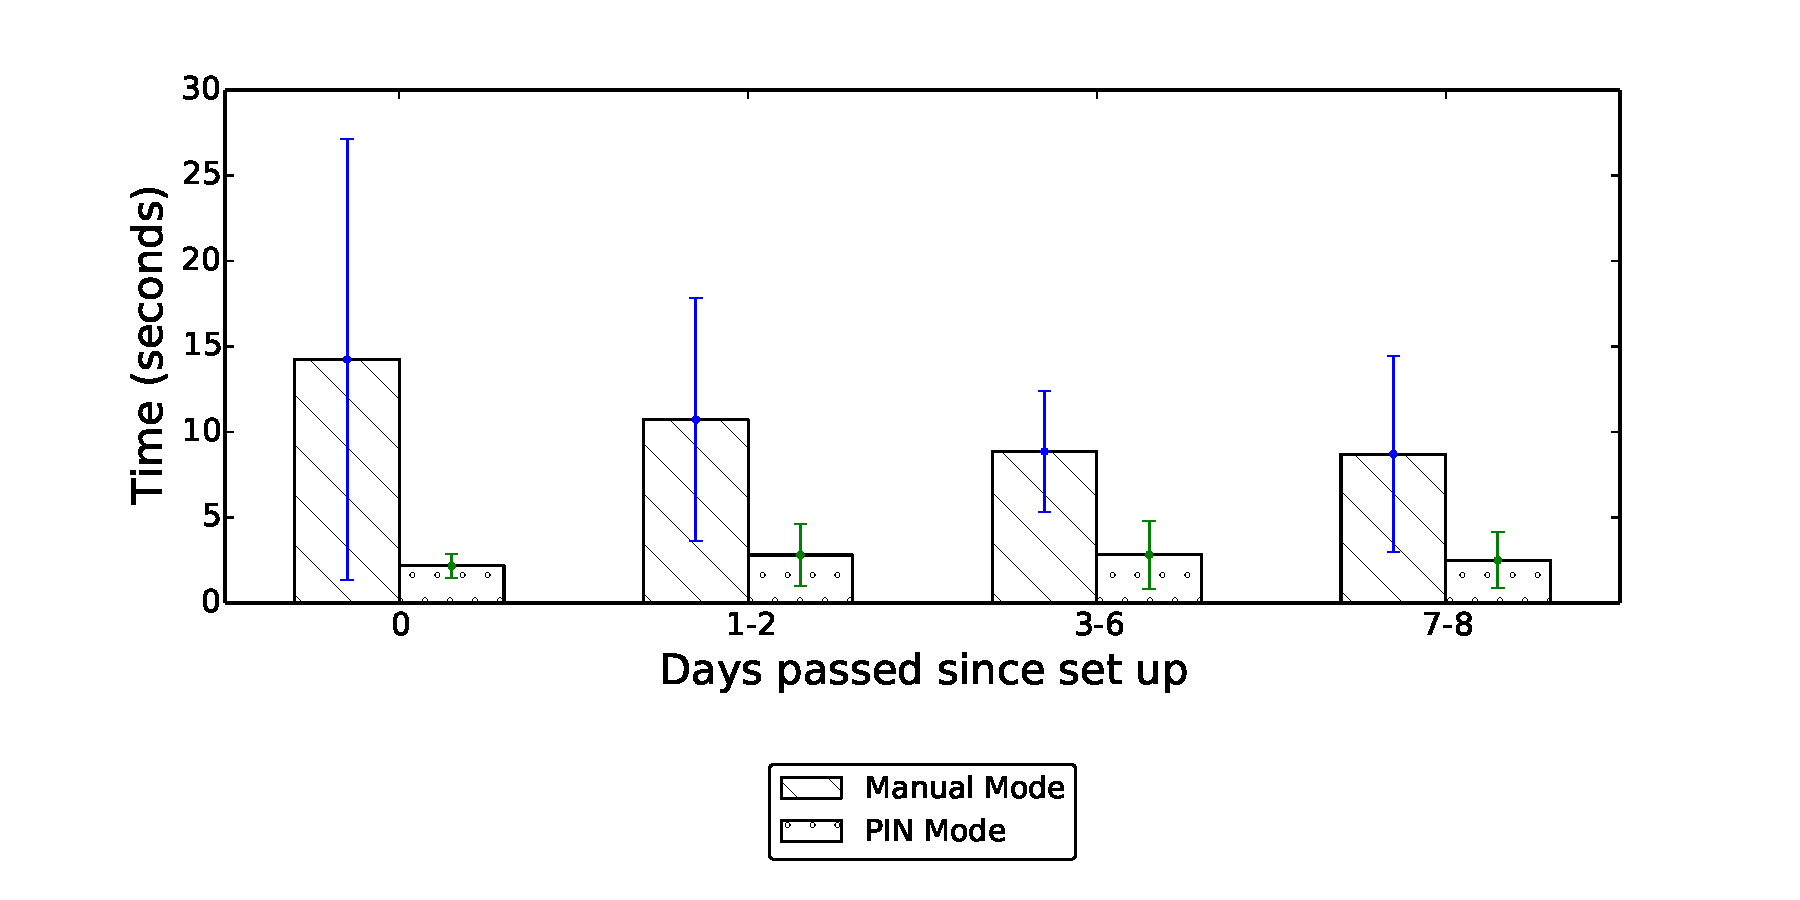
\epsfig{file=resource/ex_manual_vs_pin_time.pdf,scale=0.5}
  \end{center}
  \caption{Manual ModeとPIN Modeにおける設定時からの経過日数ごとの認証時間}
  \label{fig:ex_manual_vs_pin_time}
\end{figure}

\subsubsection{記憶保持}
表\ref{tab:manual.data}に示した通り,経過日数と認証成功率におけるピアソンの相関係数は0.8813で,標本数による限界値\cite{978-4641121607}を考慮すると有意ではないと考えられる.
また,図\ref{fig:ex_manual_vs_pin_rate}にPIN Modeとの認証率の比較を示した.
検定を行った結果,PIN Modeの認証成功率とは有意差がある(Welchのt検定,p=0.00$<$0.01)ことが明らかになった.
\begin{itemize}
  \item 短期の記憶保持
\end{itemize}
0日目から3日目までのManual Modeでの認証成功率は88.9\%から90\%と高く,標本数が少ないため,相関に関しての検定は省略する.
以上の結果から,短期の記憶保持にはあまり問題がないと考えた.

\begin{itemize}
  \item 長期の記憶保持
\end{itemize}
3日目の認証成功率は90\%で,8日目には100\%であったため,長期的な記憶保持にはあまり問題がないと考えた.
本項目も標本数が少ないため,相関に関しての検定は省略する.

\subsubsection{認証時間}
図\ref{fig:ex_manual_vs_pin_time}にManual ModeとPIN Modeとの認証時間の比較を示した.
PIN Modeとは大きく差があり,検定を行った結果,有意差がある(Welchのt検定,p=0)といえた.

\subsubsection{アンケート結果}
\begin{table}[ht]
  \begin{center}
    \small
    \begin{tabular}{|r|r|} \hline
      項目名 & 平均値 \\ \hline
      秘密情報の記憶保持にかかわる負担はどのくらい感じますか? & 2.2 \\
      認証にかかる時間はどのように感じましたか? & 3.4 \\
      認証を成功させるために必要な操作負担はどの程度でしたか? & 2.3 \\
      認証を行うのにどれくらいフラストレーションを感じましたか? & 4.2 \\ \hline
    \end{tabular}
  \end{center}
  \caption{被験者によるManual Modeに対するアンケート内評価}
  \label{tab:manual.enquete}
\end{table}
\begin{table}[ht]
  \begin{center}
    \small
    \begin{tabular}{|r|r|} \hline
      項目名 & 平均値 \\ \hline
      秘密情報の記憶保持にかかわる負担はどのくらい感じますか? & 2.2 \\
      認証にかかる時間はどのように感じましたか? & 3.4 \\
      認証を成功させるために必要な操作負担はどの程度でしたか? & 2.3 \\
      認証を行うのにどれくらいフラストレーションを感じましたか? & 4.2 \\ \hline
    \end{tabular}
  \end{center}
  \caption{被験者によるPIN Modeに対するアンケート内評価}
  \label{tab:pin.enquete}
\end{table}

\section{時系列における期間を秘密として用いることに関する評価実験}\label{sec:vsTerm}
\subsection{目的}
本実験では,SNSの情報の特性を利用した認証システムの記憶持続性と利便性の評価を行う.
更に,ある一定のルールに基づいて秘密情報が変化することが認証の成功率やユーザへの負担がどう影響を与えるかについても検証する.
また,他の実験で用いたパターンとの比較も行う.
本実験で評価対象とするパターンとして,``Auto Mode Type Term''を採用する.
アプリケーションを用いた実験で測定した指標は第\ref{sec:vsTweet}節に準ずる.

\subsection{方法}
被験者実験により各試行の成功と失敗,認証にかかった時間を収集する.
また,付録の\ref{apdx:interimEnquete}や\ref{apdx:finalEnquete}にある通り,被験者には使用パターンについて5段階のリッカート尺度を使った質問に答えてもらい,さらに既に8日間の試行が終了している他パターンとの比較もしてもらう.

\subsection{結果}
本実験の結果を述べる.
試行のタイミングが1日程度前後した被験者が存在したため,1〜2日目を1日目,3〜6日目におこなったものを3日目,7〜8日目に行ったものを8日目の試行とした.
\begin{table}[ht]
  \begin{center}
    \small
    \begin{tabular}{|r|r|r|} \hline
      経過日数 & 認証成功率(\%) & 認証時間\\ \hline
      0 & 50.00 & 23.57 \\
      1〜2 & 42.86 & 18.65 \\
      3〜6 & 85.71 & 17.43 \\
      7〜8 & 66.67 & 14.74 \\ \hline
    \end{tabular}
  \end{center}
  \caption{Auto Mode Type Termにおける各経過日数ごとの認証成功率と認証時間の変化}
  \label{tab:auto_term.data}
\end{table}

\begin{figure}[ht]
  \begin{center}
    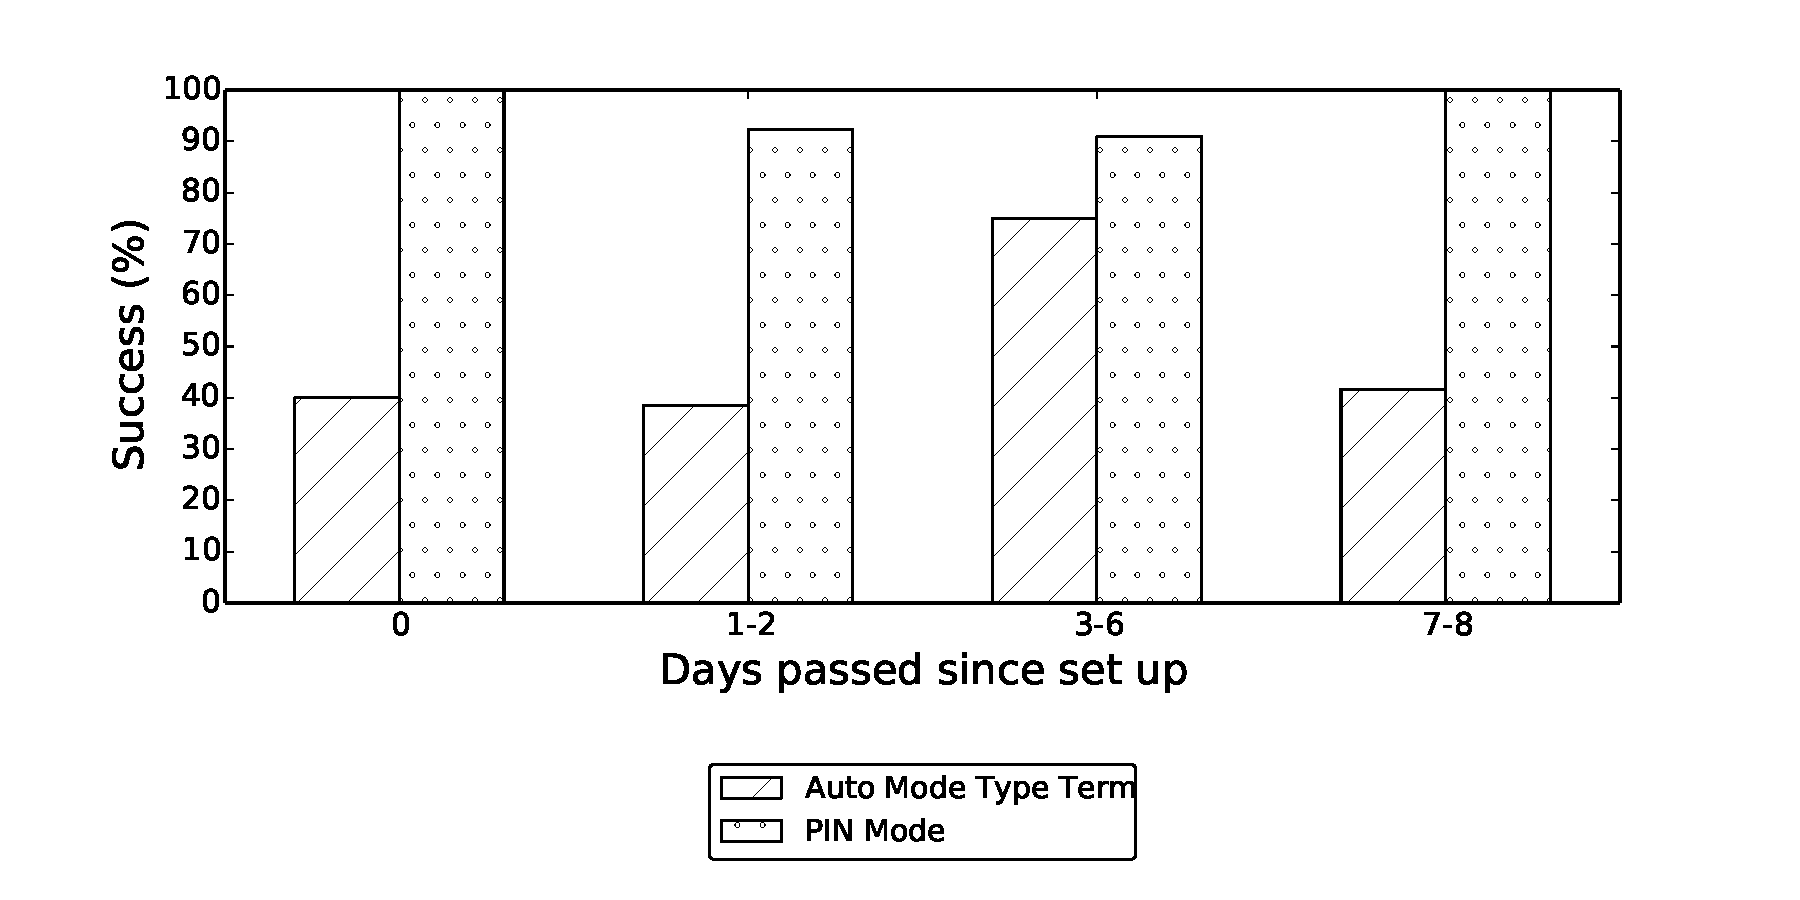
\epsfig{file=resource/ex_auto_term_vs_pin_rate.pdf,scale=0.5}
  \end{center}
  \caption{Auto Mode Type TermとPIN Modeにおける設定時からの経過日数ごとの認証成功率}
  \label{fig:ex_auto_term_vs_pin_rate}
\end{figure}

\begin{figure}[ht]
  \begin{center}
    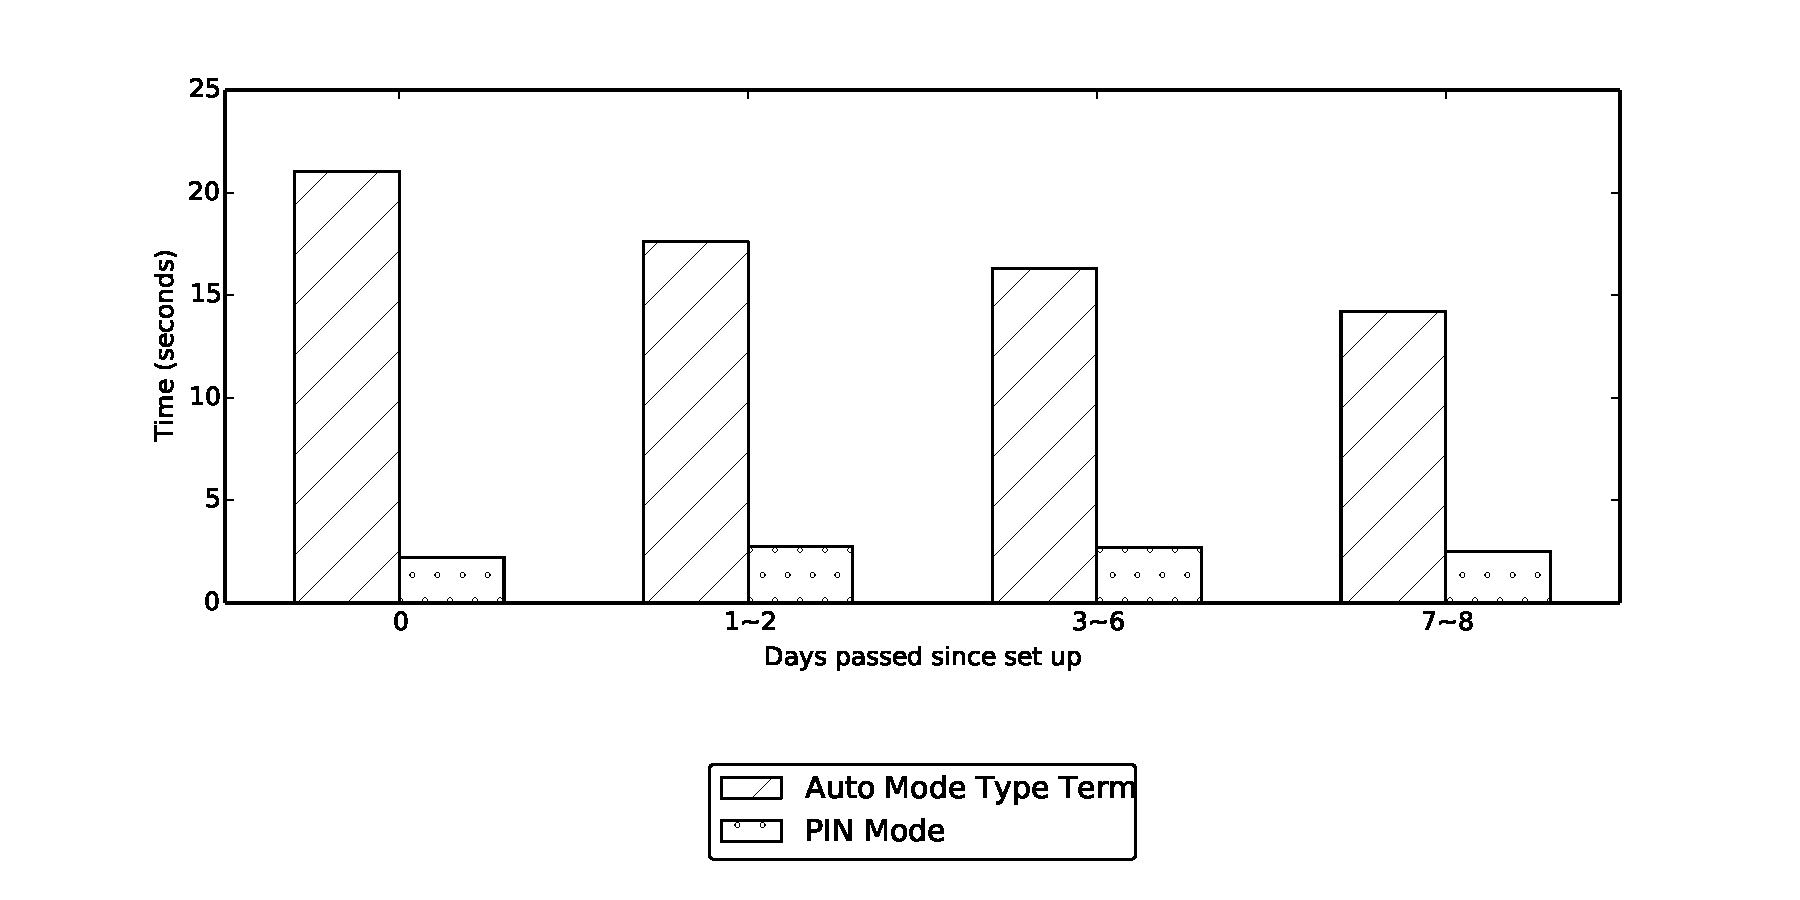
\epsfig{file=resource/ex_auto_term_vs_pin_time.pdf,scale=0.5}
  \end{center}
  \caption{Auto Mode Type TermとPIN Modeにおける設定時からの経過日数ごとの認証時間}
  \label{fig:ex_auto_term_vs_pin_time}
\end{figure}

\subsubsection{記憶保持}
表\ref{tab:auto_term.data}に示した通り,経過日数と認証成功率におけるピアソンの相関係数は0.8813で,標本数による限界値を考慮すると有意ではないと考えられる.
また,図\ref{fig:ex_auto_term_vs_pin_rate}にPIN Modeとの認証率の比較を示した.
検定を行った結果,PIN Modeの認証成功率とは有意差がある(Welchのt検定,p=0)ことが明らかになった.
\begin{itemize}
  \item 短期の記憶保持
\end{itemize}
0日目から3日目までのManual Modeでの認証成功率は50.00\%から85.71\%とばらつきが見られたが,0日目と1日目の認証成功率が低いにも関わらず3日目で上昇しているのは,設定した条件は記憶していたもののうまく候補の中から当てることが出来なかった可能性がある.
この結果に関しては標本数が少ないため,相関に関しての検定は省略する.
以上の結果から,PIN認証と比べて劣ることが明らかとなった.

\begin{itemize}
  \item 長期の記憶保持
\end{itemize}
3日目の認証成功率は85\%,8日目の認証成功率は66.67\%で,期間が空くと認証成功率が下がってしまった.
このため,長期的な記憶持続性に関しても,PINを用いたものより劣ると考えられる.
本項目も標本数が少ないため,相関に関しての検定は省略する.

\subsubsection{認証時間}
図\ref{fig:ex_auto_term_vs_pin_time}にPIN Modeとの認証時間の比較を示した.
こちらもManual Mode同様,PIN Modeとは大きく差があり,検定を行った結果,有意差がある(Welchのt検定,p=0)ことが判明した.

\subsubsection{アンケート結果}
被験者によるアンケート結果を表\ref{tab:manual.enquete}に記す.
以下の結果より,被験者にとって〜〜〜であることが考えられる.
\begin{table}[ht]
  \begin{center}
    \small
    \begin{tabular}{|r|r|} \hline
      項目名 & 平均値 \\ \hline
      秘密情報の記憶保持にかかわる負担はどのくらい感じますか? & 2.2 \\
      認証にかかる時間はどのように感じましたか? & 3.4 \\
      認証を成功させるために必要な操作負担はどの程度でしたか? & 2.3 \\
      認証を行うのにどれくらいフラストレーションを感じましたか? & 4.2 \\ \hline
    \end{tabular}
  \end{center}
  \caption{被験者によるAuto Mode Type Termに対するアンケート内評価}
  \label{tab:auto_term.enquete}
\end{table}

\section{時系列における周期を秘密として用いることに関する評価実験}\label{sec:vsCycle}
\subsection{目的}
本実験では,SNSの情報の特性を利用した認証システムの記憶持続性と利便性の評価を行う.
更に,ある一定のルールに基づいて秘密情報が変化することが認証の成功率やユーザへの負担がどう影響を与えるかについても検証する.
また,他の実験で用いたパターンとの比較も行う.
本実験で評価対象とするパターンとして,``Auto Mode Type Cycle''を採用する.
アプリケーションを用いた実験で測定した指標は第\ref{sec:vsTweet}節に準ずる.

\subsection{方法}
被験者実験により各試行の成功と失敗,認証にかかった時間を収集する.
また,付録の\ref{apdx:interimEnquete}や\ref{apdx:finalEnquete}にある通り,被験者には使用パターンについて5段階のリッカート尺度を使った質問に答えてもらい,さらに既に8日間の試行が終了している他パターンとの比較もしてもらう.

\subsection{結果}
本実験の結果を述べる.
試行のタイミングが1日程度前後した被験者が存在したため,1〜2日目を1日目,3〜6日目におこなったものを3日目,7〜8日目に行ったものを8日目の試行とした.
\begin{table}[ht]
  \begin{center}
    \small
    \begin{tabular}{|r|r|r|} \hline
      経過日数 & 認証成功率(\%) & 認証時間\\ \hline
      0 & 33.33 & 20.84 \\
      1〜2 & 20.00 & 20.42 \\
      3〜6 & 0.00 & 36.56 \\
      7〜8 & 16.67 & 24.19 \\ \hline
    \end{tabular}
  \end{center}
  \caption{Auto Mode Type Cycleにおける各経過日数ごとの認証成功率と認証時間の変化}
  \label{tab:auto_cycle.data}
\end{table}

\begin{figure}[ht]
  \begin{center}
    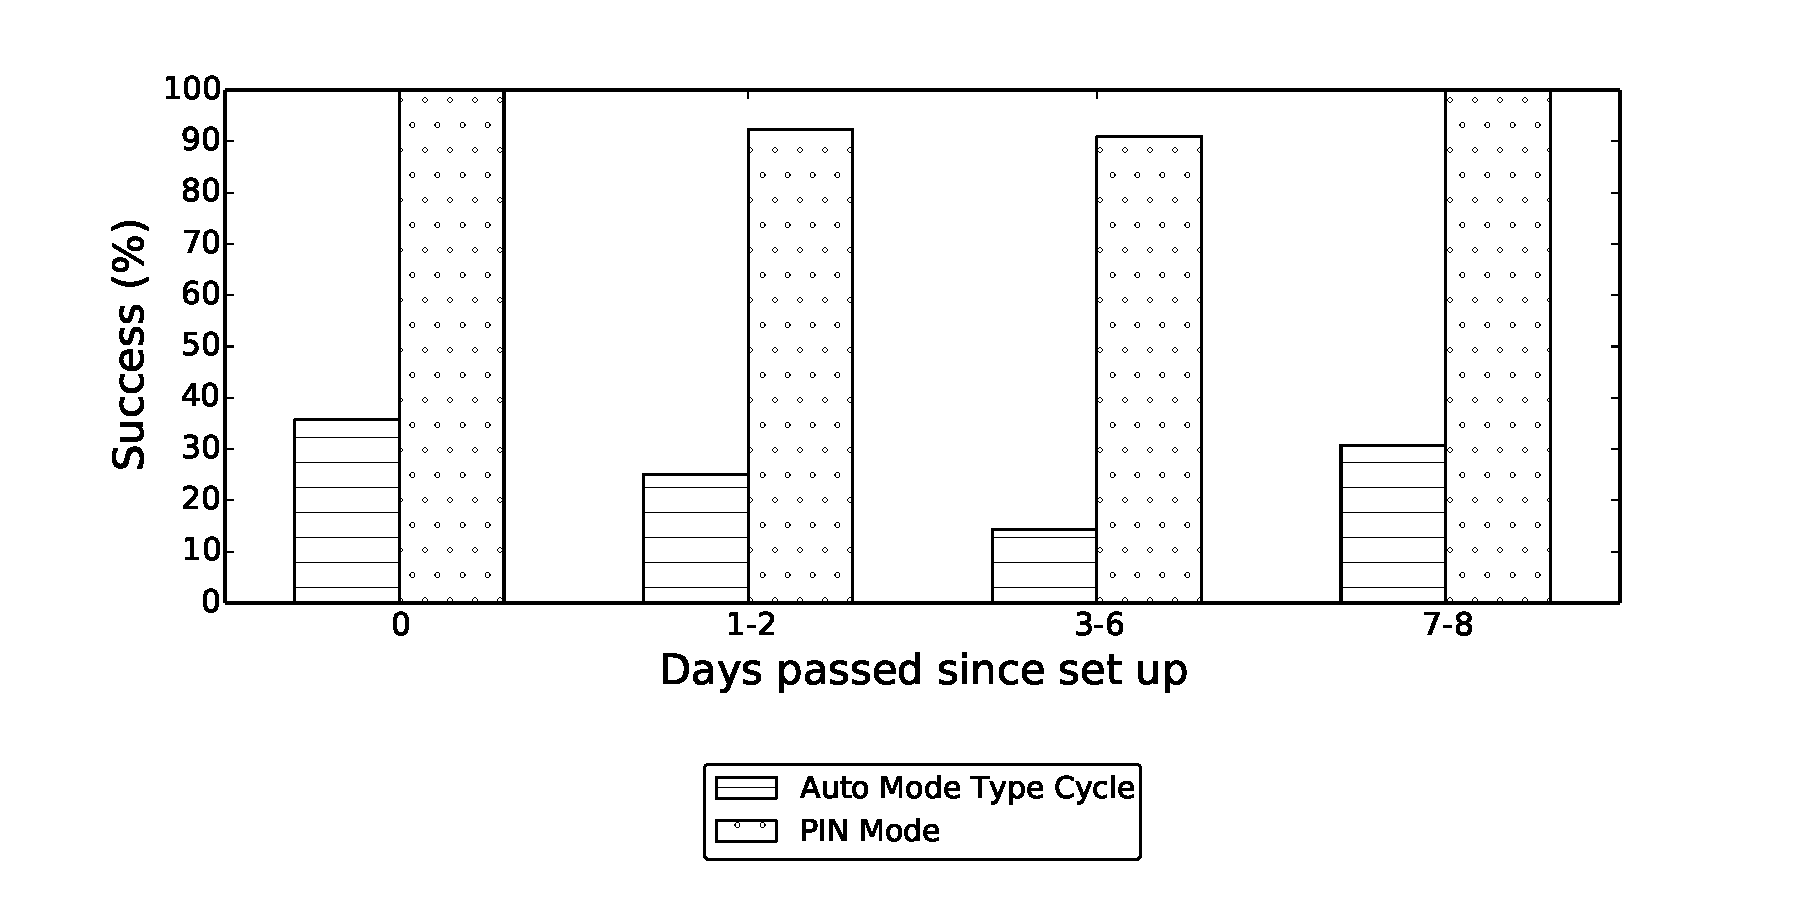
\epsfig{file=resource/ex_auto_cycle_vs_pin_rate.pdf,scale=0.5}
  \end{center}
  \caption{Auto Mode Type CycleとPIN Modeにおける設定時からの経過日数ごとの認証成功率}
  \label{fig:ex_auto_cycle_vs_pin_rate}
\end{figure}

\begin{figure}[ht]
  \begin{center}
    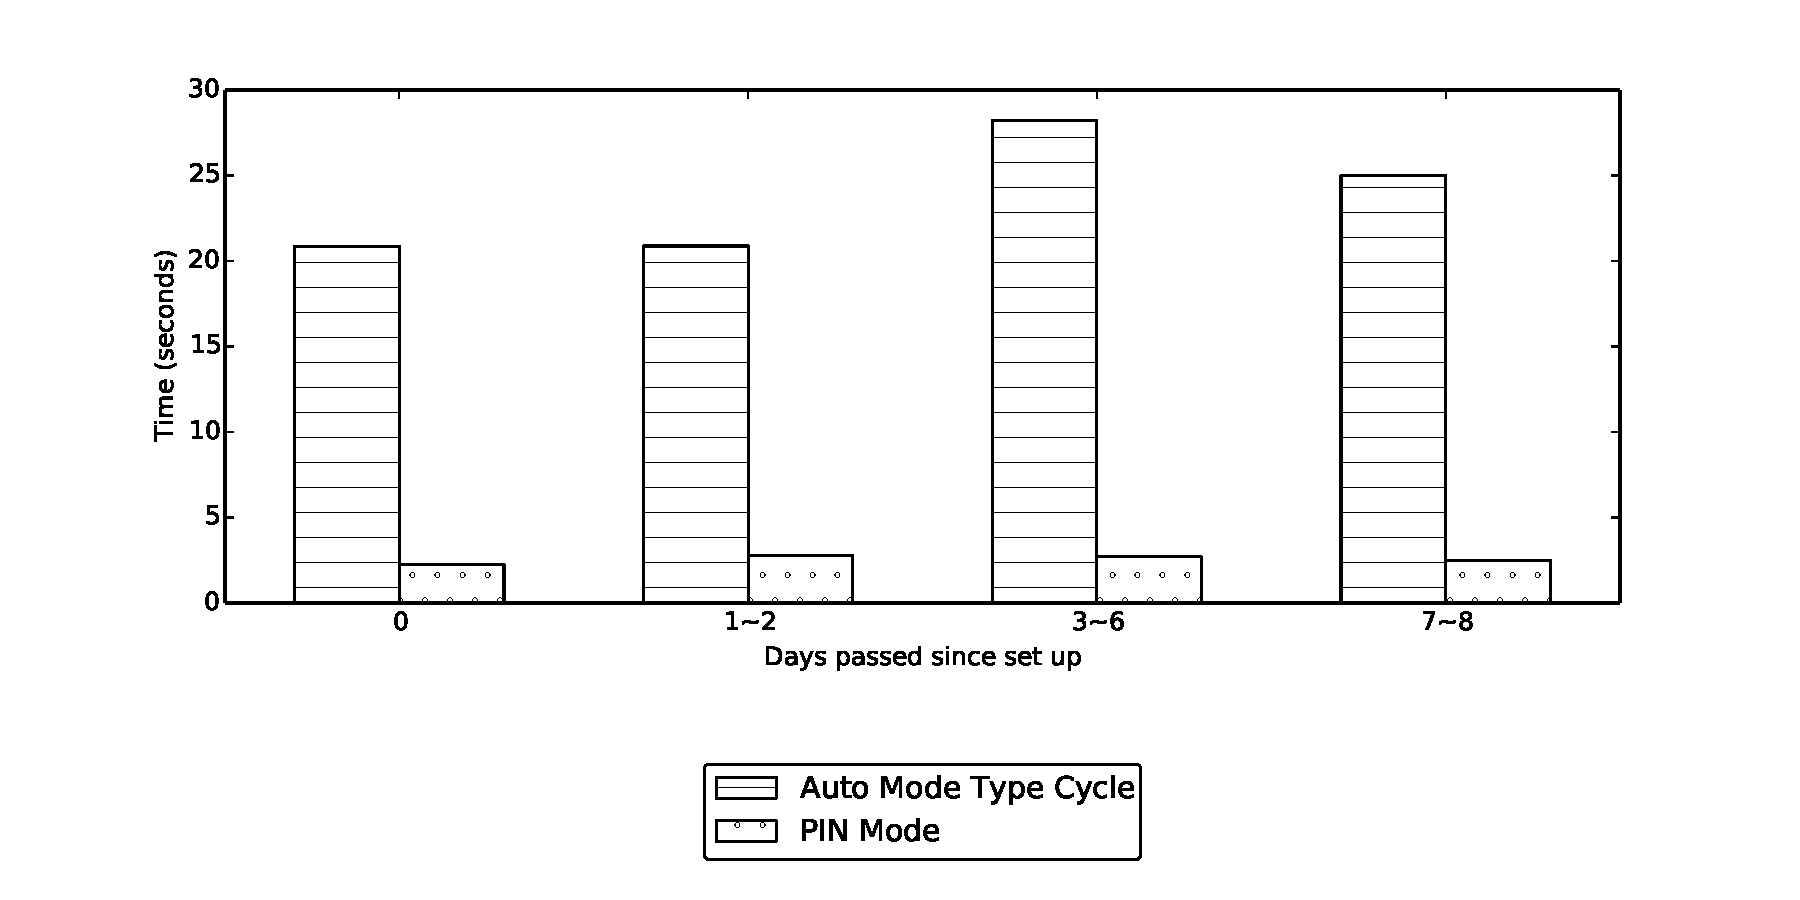
\epsfig{file=resource/ex_auto_cycle_vs_pin_time.pdf,scale=0.5}
  \end{center}
  \caption{Auto Mode Type CycleとPIN Modeにおける設定時からの経過日数ごとの認証時間}
  \label{fig:ex_auto_cycle_vs_pin_time}
\end{figure}

\subsubsection{記憶保持}
表\ref{tab:auto_cycle.data}に示した通り,経過日数と認証成功率におけるピアソンの相関係数は0.8813で,標本数による限界値を考慮すると有意ではないと考えられる.
また,図\ref{fig:ex_auto_cycle_vs_pin_rate}にPIN Modeとの認証率の比較を示した.
検定を行った結果,PIN Modeの認証成功率とは有意差がある(Welchのt検定,p=0)ことが明らかになった.
\begin{itemize}
  \item 短期の記憶保持
\end{itemize}
0日目から3日目までのAuto Mode Type Cycleにおける認証成功率は33.00\%から0\%まで落ち,一般的なPIN認証よりもかなり低く実用的ではないことが自明である.
だが,設定直後のエラー率が高いので,
この結果に関しては標本数が少ないため,相関に関しての検定は省略する.

\begin{itemize}
  \item 長期の記憶保持
\end{itemize}
3日目の認証成功率は0\%,8日目の認証成功率は16.67\%で,3日目で全員が失敗したのにその後回答に成功した被験者がいたということは,こちらも同様に設定した条件は記憶していたもののうまく候補の中から当てることが出来なかった可能性がある.
本項目においても明らかにPIN Modeよりも記憶保持の面においてが劣るが,標本数が少ないため,相関に関しての検定は省略する.

\subsubsection{認証時間}
図\ref{fig:ex_auto_cycle_vs_pin_time}にPIN Modeとの認証時間の比較を示した.
こちらも他のMode同様,PIN Modeとは大きく差があり,検定を行った結果,有意差がある(Welchのt検定,p=0)ことが判明した.

\subsubsection{アンケート結果}
被験者によるアンケート結果を表\ref{tab:auto_cycle.enquete}に記す.
以下の結果より,被験者にとって〜〜〜であることが考えられる.
\begin{table}[ht]
  \begin{center}
    \small
    \begin{tabular}{|r|r|} \hline
      項目名 & 平均値 \\ \hline
      秘密情報の記憶保持にかかわる負担はどのくらい感じますか? & 2.2 \\
      認証にかかる時間はどのように感じましたか? & 3.4 \\
      認証を成功させるために必要な操作負担はどの程度でしたか? & 2.3 \\
      認証を行うのにどれくらいフラストレーションを感じましたか? & 4.2 \\ \hline
    \end{tabular}
  \end{center}
  \caption{被験者によるAuto Mode Type Cycleに対するアンケート内評価}
  \label{tab:auto_cycle.enquete}
\end{table}

\section{各評価実験間での相互比較}\label{sec:vsAll}
\subsection{目的}
本節では,各評価実験で行ったパターン全てのなかで比較を行う.

\subsection{方法}
被験者実験により各試行の成功と失敗,認証にかかった時間を収集する.
また,付録の\ref{apdx:interimEnquete}や\ref{apdx:finalEnquete}にある通り,被験者には使用パターンについて5段階のリッカート尺度を使った質問に答えてもらい,さらに既に8日間の試行が終了している他パターンとの比較もしてもらう.

\subsection{結果}
\subsubsection{期間と周期での比較}
図\ref{fig:ex_auto_term_vs_auto_cycle_rate}と図\ref{fig:ex_auto_term_vs_auto_cycle_time}にAuto Modeの2タイプにおけるそれぞれの経過日数ごとの認証成功率と認証時間を示す.
認証の成功率に関しては,有意差は見られなかった(Welchのt検定においてp=0.067).
認証の成功時間に関しては,有意な差は見られなかった(Welchのt検定においてp=1).
この結果から,
\begin{itemize}
  \item 認証の成功率はAuto Mode Type Termの方が全日程において勝っているが,この差は有意ではない.
  \item 認証時間は大きく変わらず,差も有意ではない.
\end{itemize}
ということが判明した.

\begin{figure}[ht]
  \begin{center}
    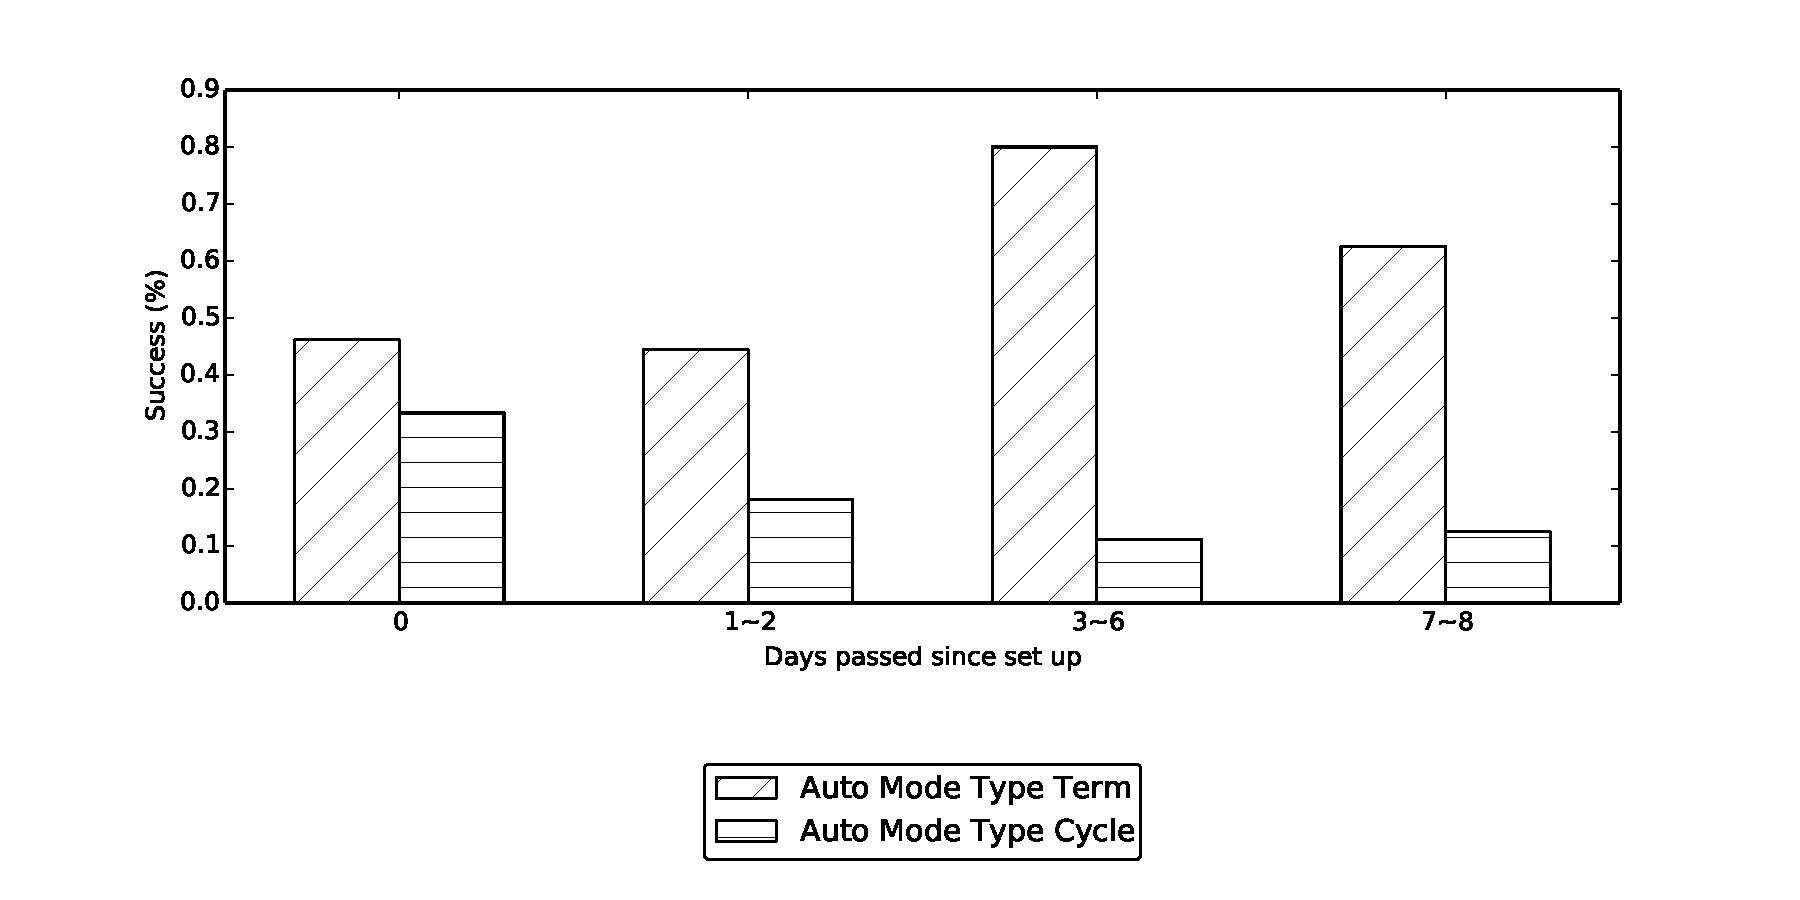
\epsfig{file=resource/ex_auto_term_vs_auto_cycle_rate.pdf,scale=0.5}
  \end{center}
  \caption{Auto Mode Type TermとAuto Mode Type Cycleにおける設定時からの経過日数ごとの認証成功率}
  \label{fig:ex_auto_term_vs_auto_cycle_rate}
\end{figure}

\begin{figure}[ht]
  \begin{center}
    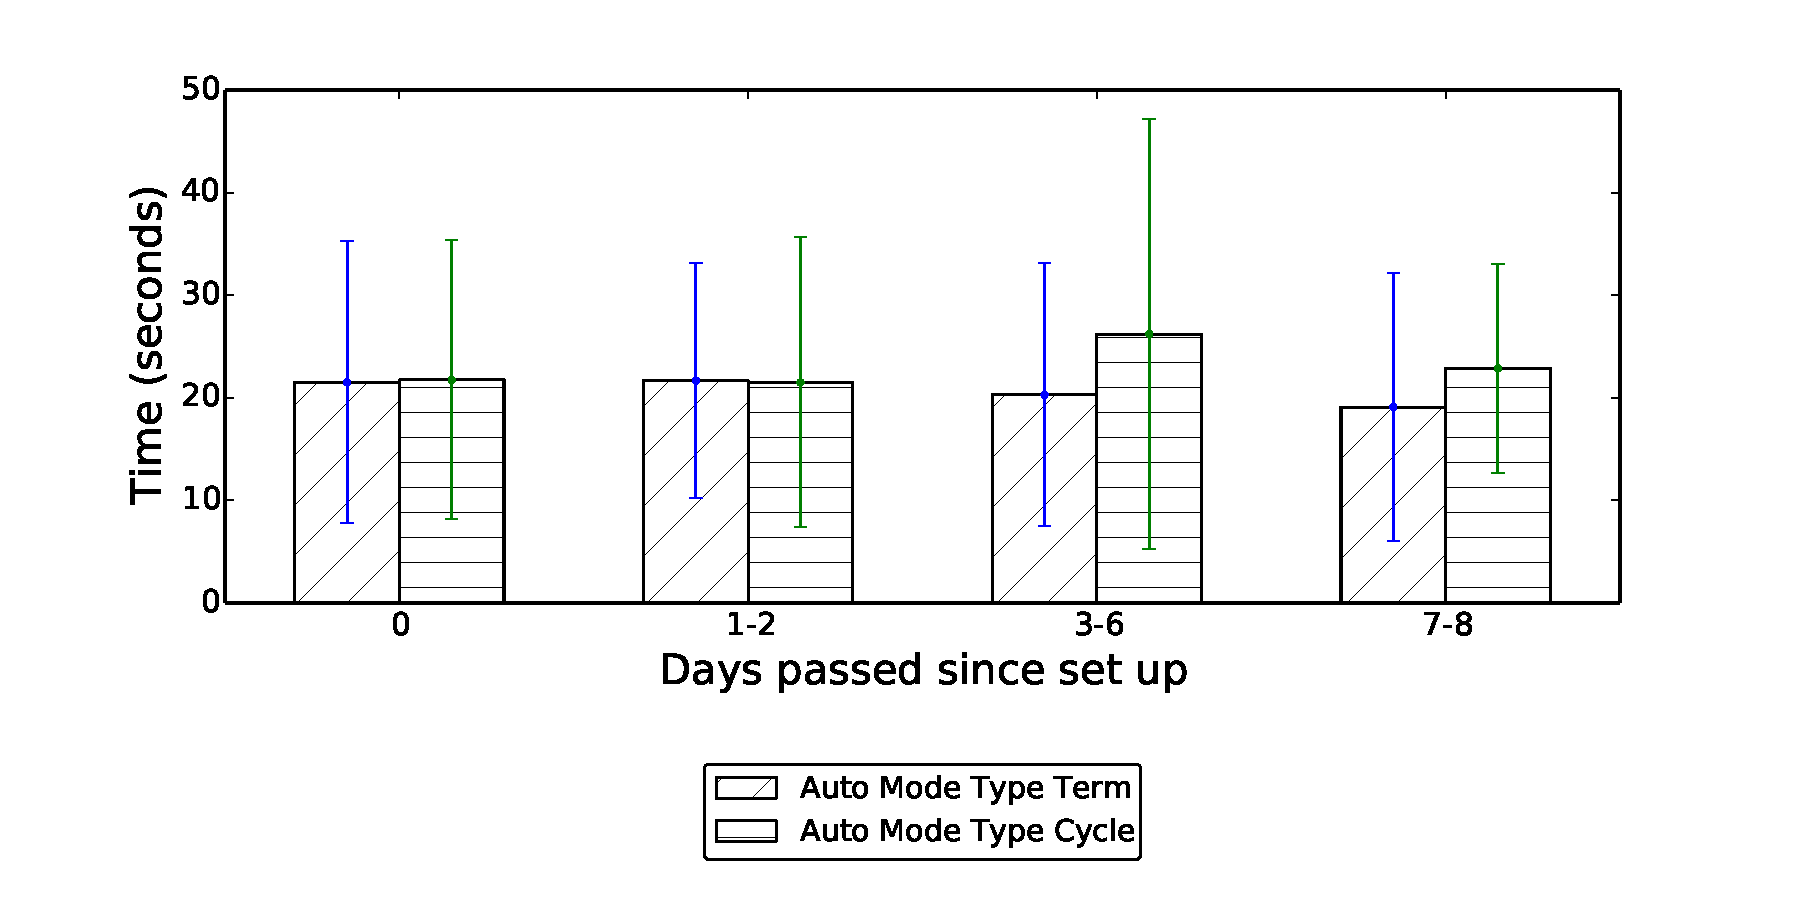
\epsfig{file=resource/ex_auto_term_vs_auto_cycle_time.pdf,scale=0.5}
  \end{center}
  \caption{Auto Mode Type TermとAuto Mode Type Cycleにおける設定時からの経過日数ごとの認証時間}
  \label{fig:ex_auto_term_vs_auto_cycle_time}
\end{figure}

\newpage

